\chapter{Reconhecimento facial}\label{cap:reconhecimento_facial}

Um sistema de reconhecimento facial é uma tecnologia capaz de realizar identificação ou verificação automática de uma pessoa através de uma imagem ou vídeo. 

Segundo \citeonline{jafri2009survey}, essas duas tarefas principais do reconhecimento facial podem ser definidas como:
%
\begin{itemize}
\item \textbf{Verificação} (correspondência um-para-um): dada uma face e uma alegação de identidade, informa se a face realmente pertence ao indivíduo.  

\item \textbf{Identificação} (correspondência de um-para-muitos): compara a imagem de uma face desconhecida com todas as imagens em um banco de dados para determinar sua identidade.
\end{itemize}

Uma terceira tarefa também importante é a de agrupamento (clustering), que consiste em agrupar faces da mesma pessoa mesmo que essa pessoa não esteja cadastrada em um banco. \cite{dhingra2017face, schroff2015facenet}.

São várias as aplicações práticas desses sistemas, como autenticação biométrica, vigilância, interação humano-computador e gerenciamento multimídia. \cite{jain2011handbook}.

O reconhecimento facial possui diversas vantagens sobre outras formas de biometria. Para validação de passaportes, por exemplo, \citeonline{heitmeyer2000biometric} afirma que esse é o método preferido por ser rápido, não intrusivo e poder ser feito à distância sem necessidade de contato.

Verificação facial em cenários cooperativos, nos quais as condições de iluminação e pose são controladas, já pode ser considerado um problema bem resolvido. Por outro lado, a identificação um-para-muitos, especialmente em cenários não cooperativos, como busca por pessoas desaparecidas ou procuradas pela polícia, ainda é uma tarefa desafiadora.
A performance do reconhecimento é grandemente influenciada por variações nas condições de iluminação, ponto de vista, poses, expressão facial, envelhecimento, uso de disfarces e acessórios \cite{li2016kernel, jain2011handbook}.

Dentre os trabalhos pioneiros em reconhecimento facial automatizado, destacam-se a tese de doutorado de Takeo Kanade em \citeyear{kanade1973picture}, os trabalhos sobre representação de faces em dimensionalidade reduzida usando PCA feitos por Kirby e Sirovich em \citeyear{sirovich1987low} e \citeyear{kirby1990application} e os trabalhos sobre Eigenfaces de Turk e Pentland em \citeyear{turk1991eigenfaces}.

Outras técnicas relevantes utilizam discriminantes lineares (Fisherfaces LDA) \cite{belhumeur1997eigenfaces, etemad1996face}, Local binary patterns \cite{ojala1994performance}, filtros de Gabor \cite{lades1993distortion, wiskott1997face, gonccalves2016robusto} e, mais recentemente, GaussianFace (DGP-LVM) \cite{lu2015surpassing} e redes neurais profundas (DNN) \cite{taigman2014deepface, he2015delving, sun2014deep, sun2014predict, sun2015deeply, zhu2014recover, schroff2015facenet, zhou2015naive, yi2014learning, sun2015deepid3, amos2016openface}.

Redes neurais profundas podem ser consideradas o estado da arte em reconhecimento facial. Com taxas de detecção acima de 99,8\% na LFW, esses métodos já ultrapassam a performance humana nesse teste \cite{learned2016labeled, kumar2009attribute}.

O processo de reconhecimento automático de faces envolve três etapas: detecção de faces, extração de características e identificação ou verificação, como ilustrado na \autoref{fig:etapas_reconhecimento}. Na fase de extração de características, é comum realizar uma normalização para alinhar as faces.

\begin{figure}[htbp]
    \caption{Etapas do reconhecimento facial}
    \label{fig:etapas_reconhecimento}
    \begin{adjustbox}{max width=\textwidth}
    \begin{tikzpicture}[
        font=\scriptsize, node distance=2cm,
        mynode/.style={draw, text width=2.5cm, align=center}
        ]
        \node[align=center] (input) {Imagem/\\Vídeo};
        \node[mynode,right=0.5cm of input] (detec) {Detecção\\Facial};
        \node[mynode,right=of detec] (extra) {Extração de\\Características};
        \node[mynode,right=of extra] (recon) {Reconhecimento\\Facial};
        \node[align=center,right=0.5cm of recon] (ident) {Identificação/\\Verificação};
        
        \draw[->,shorten <=1pt,shorten >=1pt] (input) -- (detec);
        \draw[->,shorten <=1pt,shorten >=1pt] (detec) -- node[fill=white] {Faces}(extra);
        \draw[->,shorten <=1pt,shorten >=1pt] (extra) -- node[fill=white] {Modelo}(recon);
        \draw[->,shorten <=1pt,shorten >=1pt] (recon) -- (ident);
    \end{tikzpicture}
    \end{adjustbox}
\end{figure}

Os algoritmos Eigenfaces, Fisherfaces e Local Binary Patterns Histograms (LBPH) estão implementados na biblioteca OpenCV \cite{opencvreconhecimento}.


\section{Extração de características}\label{sec:extract_caract}

Imagens digitais são representadas por milhares de pixels que são codificados em arrays de alta dimensionalidade. Os métodos de extração de características procuram encontrar as informações mais relevantes das imagens originais e representá-las em um espaço de menor dimensionalidade.

Existem $256^{10000}$ formas diferentes de formar uma imagem em tons de cinza (8 bits) de $100\times100$ pixels, mas apenas uma pequena fração dessas imagens representam faces. Além disso, muitas características são comuns a todas as faces e não são úteis para diferenciá-las.

A redução da dimensionalidade do espaço permite eliminar essas redundâncias e características indesejadas. Ela pode ser realizada se o erro quadrático médio (EQM) ou a soma da variância dos elementos são mínimas, o que é verdade para imagens de faces por elas compartilharem muitas similaridades.

Como explicado em \cite{datta2015face}, a ideia principal dos métodos de reconhecimento facial baseados em subespaço é encontrar vetores que melhor representam a distribuição de faces em todo o espaço da imagem. Esses vetores de dimensão reduzida definem o subespaço das faces. Após a linearização, o vetor médio entre todas as imagens de faces é calculado e subtraído de cada vetor correspondente às faces originais. Depois, a matriz de covariância é calculada para extrair um número limitado de autovetores, correspondentes aos maiores autovalores. Esses autovetores, também chamados eigenfaces, representam uma base em um espaço de baixa dimensionalidade. Para testar uma imagem, sua eigenface é calculada e comparada com todas as faces no banco de dados.

Os principais métodos que utilizam subespaços para reconhecimento facial são o PCA e o LDA \cite{wang2004unified}. O PCA seleciona as características que melhor representam a face e o LDA seleciona o subespaço que melhor discrimina classes de faces. Eles também podem ser utilizados em conjunto.


\subsection{Análise de componentes principais (PCA)}\label{sec:pca}

A análise de componentes principais (em inglês, principal component analysis ou PCA) é uma técnica de redução de dimensionalidade inventada em 1901 por \citeonline{pearson1901liii}.
Em \cite{gerbrands1981relationships} foi concluído que PCA é o mesmo que a transformada de Karhunen-Loève (KLT) exceto por uma possível mudança na origem do sistema de coordenadas.
Em \cite{andrews1975two} foi alertado que, apesar de próximos, SVD (decomposição em valores singulares) não é o mesmo que PCA e KLT. 

\begin{figure}[htbp]
    \caption{Análise de Componentes Principais}
    \label{fig:pca}
    \begin{subfigure}[c]{0.45\textwidth}
    \centering
    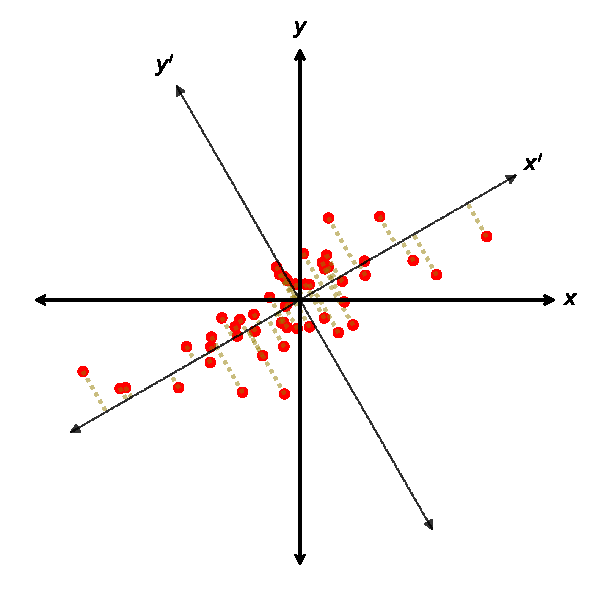
\includegraphics[width=\textwidth]{imagens/pca1.pdf}
    \caption{Distribuição original}
    \end{subfigure}
    \begin{subfigure}[c]{0.45\textwidth}
    \centering
    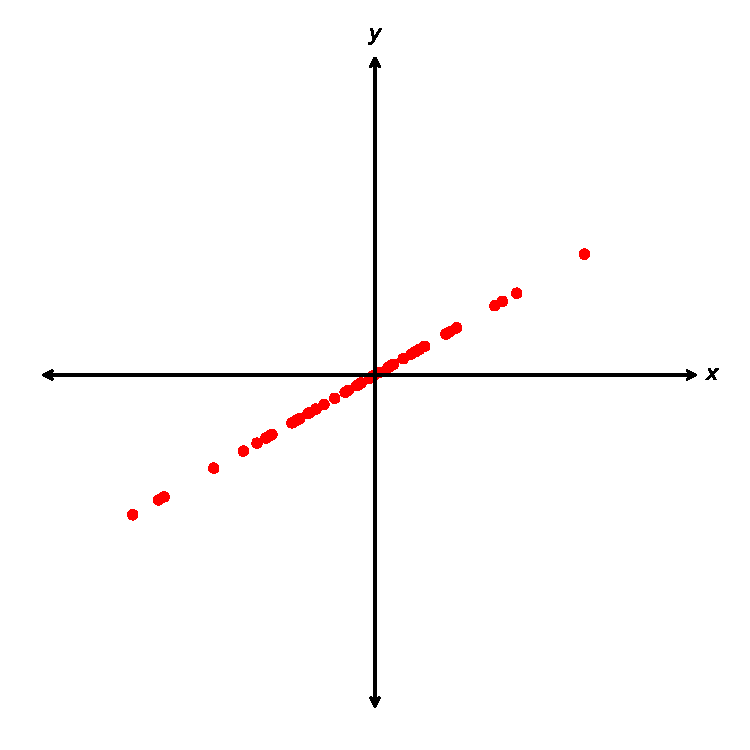
\includegraphics[width=\textwidth]{imagens/pca2.pdf}
    \caption{Apenas o primeiro componente principal}
    \end{subfigure}
\end{figure}

Segundo \cite{jolliffe2002principal}, a ideia central da análise de componentes principais (PCA) é reduzir a dimensionalidade de um conjunto de dados que consiste em um grande número de variáveis, mantendo o máximo possível a variação presente no conjunto de dados. Isto é alcançado através da transformação para um novo conjunto de variáveis,
os componentes principais, que não são correlacionados, são
ordenados de forma que os primeiros retenham a maior parte da variação presente em todas as variáveis originais.

O conceito do PCA está ilustrado na \autoref{fig:pca}. Os eixos $x$ e $y$ formam a base original; o eixo $x'$ corresponde à direção de maior variância, ou seja, ao primeiro componente principal.

Matematicamente, dados $n$ pontos em $\mathbb{R}^p$, a PCA consiste em escolher uma dimensão $k < p$ e encontrar um espaço afim de dimensão $k$ onde a distância ao quadrado dos pontos às suas projeções ortogonais no espaço são minimizadas.


\subsection{Eigenfaces}\label{sec:eigenfaces}

As eigenfaces são os componentes principais de uma distribuição de faces, ou seja, os autovetores da matriz de covariância de um conjunto de imagens de faces.
Cada face pode ser representada como uma combinação linear de eigenfaces. Elas também podem ser aproximadas usando apenas as eigenfaces que possuem os maiores autovalores e que, consequentemente, são responsáveis pela maior variância.

A ideia de usar componentes principais para representar faces humanas foi desenvolvida por \citeonline{sirovich1987low} e usada por \cite{turk1991eigenfaces} para detecção e reconhecimento facial.
Muitos consideram essa técnica de reconhecimento facial baseada em aparência como a primeira a ser utilizada com sucesso na prática.

O algoritmo para a obtenção das eigenfaces proposto em \cite{turk1991face} pode ser formulado da seguinte forma:

\begin{enumerate}
    \item Obter $M$ imagens $I_1, I_2, I_3 \ldots I_M$ com dimensão $N \times N$.
    As imagens devem estar centralizadas.
    \item Representar cada imagem $I_i$ como um vetor $\Gamma_i$ de dimensão $N^2 \times 1$.
    %
    \begin{equation} \label{eq:eign_gamma}
        \begin{bmatrix}
        a_{11} & a_{12} & \cdots & a_{1N}\\ 
        a_{21} & a_{22} & \cdots & a_{2N}\\ 
        \vdots & \vdots & \ddots & \vdots\\ 
        a_{N1} & a_{N1} & \cdots & a_{NN}
        \end{bmatrix}_{N \times N} \rightarrow \begin{bmatrix}
        a_{11}\\ 
        \vdots\\ 
        a_{1N}\\ 
        \vdots\\ 
        a_{2N}\\
        \vdots\\ 
        a_{NN}
        \end{bmatrix}_{N^2 \times 1}
    \end{equation}
    %
    \item Calcular o vetor $\Psi$ correspondente à face média.
    %
    \begin{equation} \label{eq:eign_media}
        \Psi = \frac{1}{M}\sum_{i=1}^{M}\Gamma_i
    \end{equation}
    %
    \item Subtrair a face média de cada vetor $\Gamma_i$ para obter o conjunto de vetores $\Phi_i$.
    %
    \begin{equation} \label{eq:eign_phi}
        \Phi_i = \Gamma_i - \Psi
    \end{equation}
    %
    \item Encontrar a matriz $C$ de covariância.
    %
    \begin{equation} \label{eq:eign_c}
        C = AA^T \text{, onde } A = \begin{bmatrix}\Phi_1  & \Phi_2 & \ldots  & \Phi_3\end{bmatrix}
    \end{equation}
    %
    $C$ é uma matriz $N^2 \times N^2$ e $A$ é uma matriz $N^2 \times M$.
    \item Calcular os autovetores $u_i$ de $C = AA^T$.
    
    Em vez desse cálculo, que resultaria em $N^2$ autovetores, calcular os autovetores $v_i$ da matriz $A^TA$ de dimensão $M \times M$.
    %
    \begin{equation} \label{eq:eign_autov}
    \begin{alignedat}{2}
                     && A^T Av_i    &= \mu_i v_i\\
    \Rightarrow\quad && AA^T Av_i   &= \mu_i Av_i\\
    \Rightarrow\quad && CAv_i       &= \mu_i Av_i\\
    \Rightarrow\quad && u_i         &= Av_i
    \end{alignedat}
    \end{equation}
    %
    ou seja, $Av_i$ são autovetores de $C = AA^T$. Os $M$ autovalores de $A^TA$ correspondem aos $M$ maiores autovalores de $AA^T$.
    \item Manter apenas os $K$ autovetores, correspondentes aos $K$ maiores autovalores.
\end{enumerate}

Cada face $\Phi_i$ (face menos a média) correspondente a uma das $M$ imagens de treinamento possui uma representação vetorial $\Omega_i$ na base formada pelos $K$ autovetores escolhidos, ou seja, pode ser representada pela seguinte combinação linear:
%
\begin{equation} \label{eq:eign_lincomb}
    \Gamma_i - \Psi = \Phi_i = \sum_{j=1}^{K}w_ju_j, (w_j = u_{j}^{T}\Phi_i)
\end{equation}
%
Cada peso $w_j$ descreve a contribuição do autovetor $u_j$ na representação da imagem. Eles formam o seguinte vetor $\Omega_i$:
%
\begin{equation} \label{eq:eign_lincomb_vetor}
\Omega_i = \begin{bmatrix}
        w_{1}^{i}\\ 
        w_{2}^{i}\\ 
        \vdots\\ 
        w_{K}^{i}
        \end{bmatrix}, i = 1, 2, \ldots, M
\end{equation}
%

\begin{figure}[htbp]
    \centering
    \caption{Representação de uma face como combinação linear de eigenfaces}
    \label{fig:eign_lincomb}
    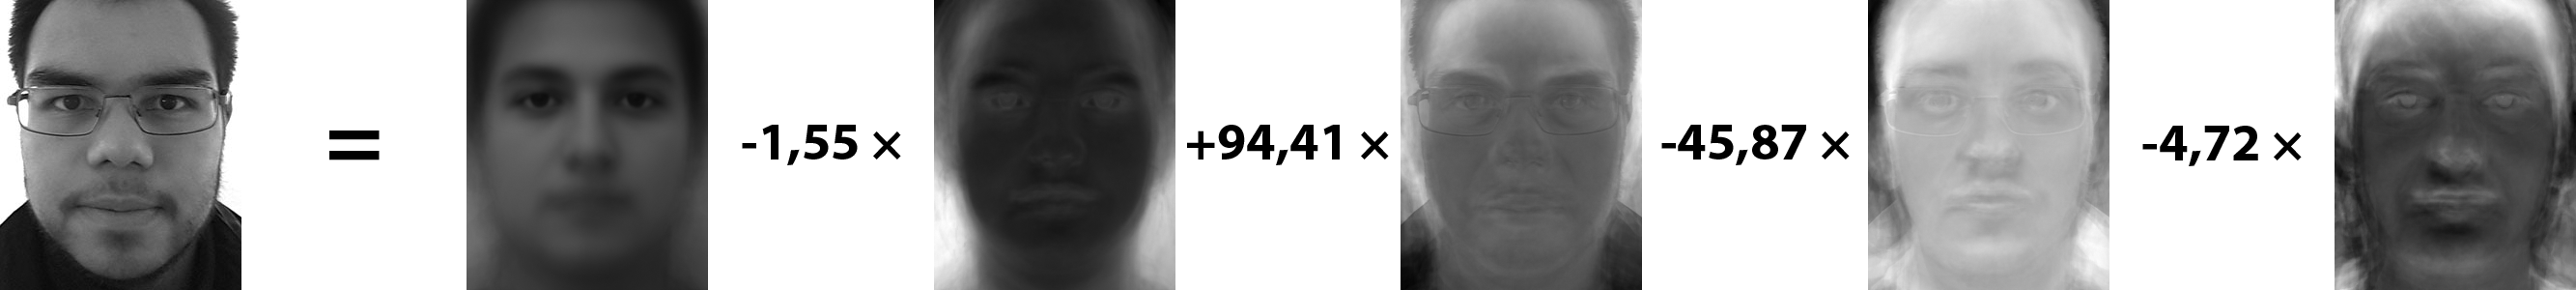
\includegraphics[width=0.95\linewidth]{imagens/eign_lincomb.png}
\end{figure}

O reconhecimento de uma face desconhecida $\Gamma$ centralizada e com as mesmas dimensões das imagens de treinamento é feito através os seguintes passos:

\begin{enumerate}
    \item Normalizar a imagem.
        \begin{equation} \label{eq:eign_rec_norm}
            \Gamma: \Phi = \Gamma - \Psi
        \end{equation}
    \item Projetar no autoespaço.
        \begin{equation} \label{eq:eign_rec_lincomb}
            \hat{\Phi} = \sum_{i=1}^{K}w_iu_i, (w_i = u_{i}^{T}\Phi)
        \end{equation}
    \item Representar $\Phi$ como $\Omega$:
        \begin{equation} \label{eq:eign_rec_omg}
            \Omega = \begin{bmatrix}
            w_{1}\\ 
            w_{2}\\ 
            \vdots\\ 
            w_{K}
            \end{bmatrix}
        \end{equation}
    \item Calcular a distância $e_r = min_l\left \| \Omega - \Omega^l \right \|$.
    \item Se $e_r < T_r$, então $\Gamma$ é reconhecida como a face l do conjunto de treino.
\end{enumerate}


\begin{figure}[htbp]
    \centering
    \caption{Eigenfaces}
    \label{fig:eigenfaces_faces}
    \begin{subfigure}[t]{0.3\textwidth}
    \centering
    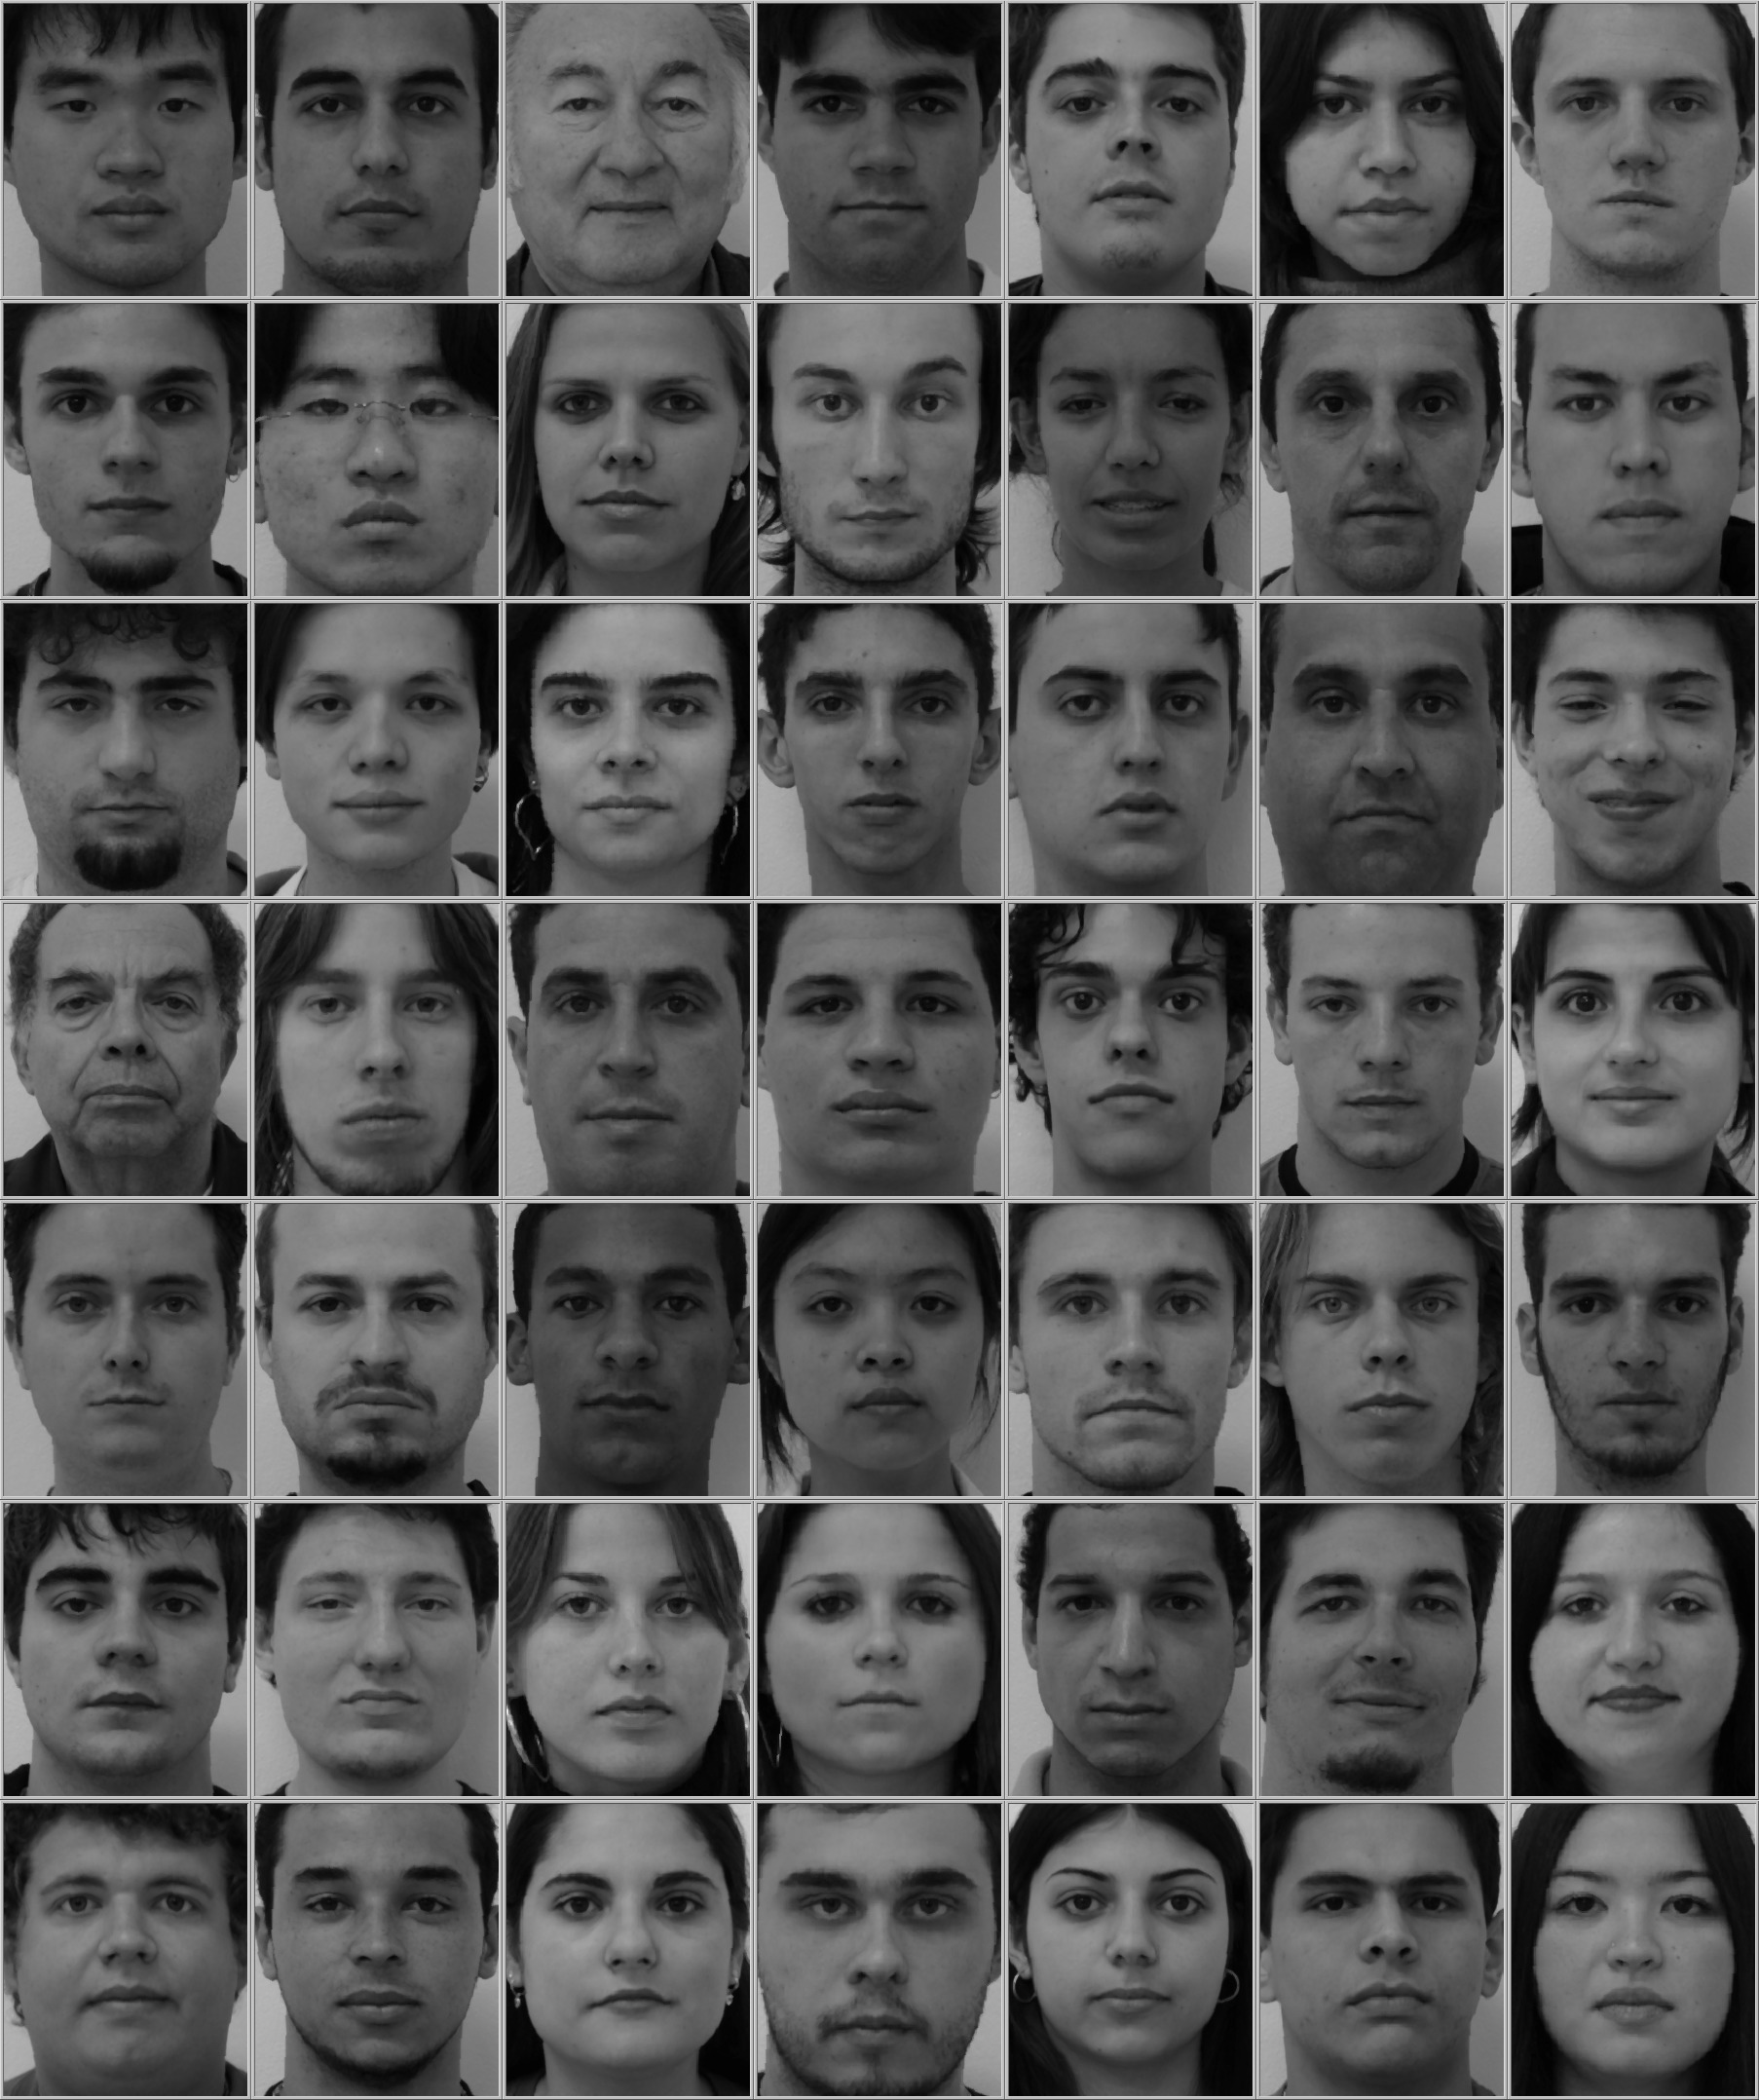
\includegraphics[width=\textwidth]{imagens/faces_fei.jpg}
    \caption{Algumas das faces da FEI Face Database}
    \end{subfigure}
    \begin{subfigure}[t]{0.3\textwidth}
    \centering
    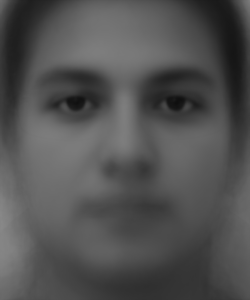
\includegraphics[width=\textwidth]{imagens/face_media.png}
    \caption{Face média}
    \end{subfigure}
    \begin{subfigure}[t]{0.3\textwidth}
    \centering
    
\includegraphics[width=\textwidth]{imagens/eigenfaces.png}
    \caption{Eigenfaces}
    \end{subfigure}
\end{figure}

O \autoref{cod:eigenfaces_opencv} apresenta como realizar o reconhecimento facial com Eigenfaces utilizando a biblioteca OpenCV. O resultado da execução usando o banco de faces AT\&T pode ser visto na \autoref{fig:eigenfaces_resultado}.

\begin{figure}[htbp]
    \centering
    \caption[Teste do algoritmo Eigenfaces]{Teste do algoritmo Eigenfaces (\autoref{cod:eigenfaces_opencv}). Em verde as detecções corretas, em vermelho as erradas}
    \label{fig:eigenfaces_resultado}
    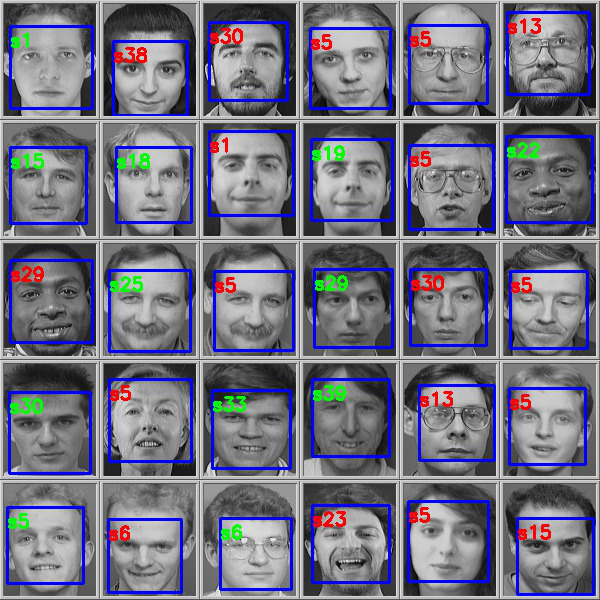
\includegraphics[width=0.95\linewidth]{imagens/eigenfaces_resultado.jpg}
\end{figure}

